\documentclass[a4paper,twocolumn,10pt]{jsarticle}

\usepackage{geometry}
\geometry{top=20mm, bottom=24mm, left=23mm, right=23mm}

\makeatletter
  % maketitle
  \def\@maketitle{%
    \newpage
    \begin{center}%
     %和文題名
     {\Large \textbf{\@title} \par}%
     \vskip 9pt
     %和文著者
     {\large \lineskip .0em
     \begin{tabular}[t]{c}%
      \@author
     \end{tabular} \par}%
     %英文題名
     \vskip 1.5em
     {\Large \textbf{\etitle@etitle} \par}%
     \vskip 0.5em
     %英文著者
     {\large \lineskip .0em
     \begin{tabular}[t]{c}%
      \etitle@eauthor
     \end{tabular} \par}%
     \vskip 0.5em
    \end{center}%
    \par\vskip 1.5em
    \ifvoid\@abstractbox\else\centerline{\box\@abstractbox}\vskip1.5em\fi
    }
  % \title \author は既存のマクロを利用 \@title \author に値がセットされる.
  \newcommand{\etitle@etitle}{}
  \newcommand{\etitle@eauthor}{}
  \newcommand{\affiliation}[1]{\renewcommand{\etitle@affiliation}{#1}}
  \newcommand{\etitle}[1]{\renewcommand{\etitle@etitle}{#1}}
  \newcommand{\eauthor}[1]{\renewcommand{\etitle@eauthor}{#1}}
\makeatother

% !!!重要!!! ファイル先頭からこの行までの間は改変しないこと.

% 必要に応じて適宜パッケージを追加
% 例:特殊な数学記号を利用する→ \usepackage{amsmath} など
\usepackage[dvipdfmx]{graphicx}  % 図をインポートするパッケージ
\usepackage{url}       % URLを \url{} で括ると見やすくなる

% 和文題名
\title{宮下ゼミ卒業論文テンプレート2024}
% 和文著者
\author{京都女子大学 現代社会学部 現代社会学科 宮下ゼミ\\
21241000 西本 願子}
% 英文題名
\etitle{Manuscript Template for Graduation Thesis in Miyashita Lab 2024}
% 英文著者. 和文所属と同様です
\eauthor{Miyashita Lab., Faculty for the Contemporary Society, Kyoto Women's University\\
21241000 Nishimoto Ganko}

% 論文の概要
\begin{abstract}
本稿は京都女子大学現代社会学部宮下ゼミの学生向けに書かれた卒業論文のテンプレートであり,同時に卒業論文執筆の際の注意点などをまとめたものでもある.
主に \LaTeX の使い方に関する説明と,論文の内容に関して``するべきこと''と``するべきでないこと''をまとめている.
本稿自体も \LaTeX を利用して執筆されているので,卒業論文作成の参考になれば幸いである.
さて,本来この部分には卒業論文の概要(論文内容を簡潔にまとめたもの)を書く.
つまり研究の動機や背景,問題,解決手法,結論などを簡潔にまとめた文章を「概要」としてまとめる.
この概要を読めば論文内容がだいたい示されているようにすることが重要である(もともと「概要」とはそのようなものである).
文章量は特に定めないが,だいたい6〜8行程度にすればバランスがよいと思われる.
\end{abstract}

\begin{document}
% \begin{document} 直後に \maketitle コマンドを置く
\maketitle

\section{はじめに}
\label{hajimeni}

これは京都女子大学現代社会学部現代社会学科宮下ゼミ(以下,本ゼミという)の学生向けに書かれた卒業論文テンプレートである\footnote{このテンプレートの最新版は\url{https://github.com/kensuke-m/graduationthesis-template}から入手できる.}.
本ゼミの学生はこの内容をよく理解し,すばらしい卒業論文を執筆していただきたい.
また,このテンプレートに足りないところや誤りがあればいつでも指摘してほしい.

本稿ではまず\LaTeX のスタイルファイルを用いた論文のフォーマットについて述べる.
論文フォーマットについて詳しくは\ref{sec:format}節で後述する指針を参照してほしい.
また,そこで説明されていることの外は標準的な \LaTeX のコマンドや他のスタイルファイルなどを利用して構わない.
これまでレポート作成などで利用してきた Microsoft Word ではない環境での文書作成を楽しんでもらえれば幸いである.
本稿自身も卒業論文のテンプレートとして実際に \LaTeX を利用しているので,論文執筆時にはソースファイル({\tt main.tex})なども参考にされたい.

また,卒業論文を執筆する際に著者(これを読んでいるあなたである)がするべきこと,するべきでないこともまとめてある.
本稿の後半ではこれらについて指針を述べているので,卒業論文提出前はもとより執筆中にもぜひ継続的にチェックしていただきたい.
ただし卒業研究自体については本稿には何も書かれていない.
研究はゼミで指導した通り,各自で進めてほしい.

さて,明確で簡潔に書かれた文書に勝るものはない.
第2次大戦中,イギリスのウィンストン・チャーチル首相は「我が国の外務省は長い報告書を書けばナチスに勝てると思っているようだ」としばしばこぼしたという\cite{newsweek2021}.
卒業論文(に限らず他人に読んでもらうことが目的の文書はすべてそうだが)は,できる限り短く,論旨が明確で,理解しやすいものを目指そう.

\section{卒業論文執筆の流れ}

卒業論文は以下のように執筆し,提出することが望ましい.

\subsection{準備}

このテンプレートには以下のファイルが含まれている.
\begin{enumerate}
 \item \verb|graphs.png    |: 図で利用する画像ファイル
 \item \verb|ipsjunsrt.bst |: 参考文献リスト設定ファイル
 \item \verb|latexmkrc     |: \LaTeX の設定ファイル
 \item \verb|main.tex      |: 本稿のソースファイル
 \item \verb|README.md     |: 利用法の説明
 \item \verb|reference.bib |: 参考文献リスト
\end{enumerate}
参考文献リスト設定ファイルは,情報処理学会\LaTeX スタイルファイル\footnote{\url{https://www.ipsj.or.jp/journal/submit/style.html}}から引用している.
ここに記して感謝する.

卒業論文はこのファイルのように文書処理システム \LaTeX を利用して作成し,PDF形式で提出する.
以前は \LaTeX を各自がPCにインストールして利用していたが,近年ではWWW上のアプリケーションとして利用するOverleaf\footnote{\url{https://ja.overleaf.com}}のようなシステムが普及しているので,それを使うことを想定している\footnote{もちろん,自分のPCにインストールしたい人を止めたりはしないが,それによる問題の発生などには対処し切れないので,ある程度覚悟を決めてかかるように.}.

\subsection{執筆}

本稿にしたがって卒業論文を執筆し,\LaTeX ソースファイルからPDFファイルを作成する.
前述した Overleaf では「リコンパイル」ボタンをクリックするか,または Alt キーを押しながら Return キーを押下することでPDFファイルが作成され,WWWブラウザ内でプレビューできる.
その際エラーが発生すれば適宜修正し\footnote{ここでは具体的なエラーの説明はしない.エラーメッセージ自体をキーワードとして検索すれば大抵の場合は対処法がヒットする.},めでたくプレビューできた場合は自分の意図通りの体裁になっているか,誤字や脱字などはないかなどをチェックする.
そして説明の足りないところを補ったり,図表を挿入してわかりやすくしたりなどの改善を繰り返しつつ,卒業論文を完成に近づけよう.

ある程度執筆が進んだらPDFファイルをダウンロードして紙に印刷してみることをお勧めする.
PCのディスプレイやタブレットなどの透過光で読む原稿と紙に印刷して反射光で読む原稿では見え方が異なり,一方では気付かなかったことに他方で気付くことが多い.
特に,最終的に完成した(と思われる)卒業論文を提出する直前には印刷したものを一度通して読んでみると良い.

自分では現時点でこれ以上改善すべき箇所が見当たらないというところまで来たら,AIにチェックさせたり信頼のおける人に読んでもらったり,または教員に提出したりしてコメントをもらおう.
自分では気付かなかったことが必ずあるはずで,そういうところが何か所も指摘されるはずである.
指摘をもとに自分で考え,文章や構成を改善しよう.

卒業論文提出までにこのようなやりとりを何度も繰り返し,より良い論文を作成してほしい.

\subsection{提出}

本ゼミでは卒業論文を提出する際に,ゼミ内での提出と教務課への提出の2つが要求される.
もちろん両方が必要である.

前者では,PDF形式のファイルを教員が指定した方法で然るべき場所へアップロードする.
具体的には,Microsoft Teams内のその年度の演習VIのチャネルに「卒業論文」という課題が作成されるので,そこへPDFファイルをアップロードする.

後者は,京女ポータル内のコミュニティへPDFファイルを提出するのが通例である.
このとき,卒業論文題目というフォームにも記入する必要があり,これは京女ポータル上で卒業論文のタイトルや指導教員名などを入力するものである.
このあたりに関する情報は京女ポータルに掲載されるので,秋が深まって来たら京女ポータルの「お知らせ」に注意すること.

どちらも2025年1月15日(水)17時が〆切であるが,少し余裕を持って提出できるよう計画すると良い\footnote{京女ポータルでは毎年12月後半から受け付けてもらえるようである.}.

\section{卒業論文フォーマット}
\label{sec:format}

卒業論文は電子的な媒体で読む(例えばPCやタブレットの画面で閲覧する)のに適するよう作成し,PDF形式のファイルで提出する.
以下では卒業論文のフォーマットについて指針を述べるので,これにしたがって執筆すること.
\LaTeX を利用した文書作成について一般的な知識は \cite{okumura2020} などの書籍を参考にされたい.

\subsection{卒業論文の構成}

卒業論文の \LaTeX ソースファイル({\tt main.tex})の構成は以下のようになる.

まず,ファイルの冒頭から\\
\verb|% !!!重要!!! ファイル先頭からこの行までの間は改変しないこと.|\\
と書かれた行までは改変せずそのまま利用する.

上記の行の直下には利用したい \LaTeX パッケージを列挙する.
図をインポートするのに便利な graphicx とURLを扱いやすくするための url パッケージを,例も兼ねてインクルードするように記述してあるので,他に必要なパッケージがあればそれらに倣うと良い.

その後,\verb|\title{表題(和文)}| と \verb|\author{著者(和文)}| および \verb|\etitle{表題(英文)}| と \verb|\eauthor{著者(英文)}| を例に倣って記述する.
表題は論文内容を端的に表すものとし,通常は体言止めとする\footnote{他の分野では表題の次に``〜○○の観点から〜''のような副題を追記することがあるが,情報系分野ではあまり見かけないのでこのような形式は避ける方が良い.}.
表題は少し大きな字でセンタリングして出力される.
長い表題は自動的に改行されるが,適切と思う箇所に \verb|\\| を挿入しても良い\footnote{このような意図的な改行は表題以外(例えば本文)ではできるだけ行わないこと.}.
著者の所属は例のままとし,学生証番号と氏名を自分のものに変更する.
英文の表題は和文のものを翻訳し,英文の著者はローマ字で綴る.

\verb|\begin{abstract}| から \verb|\end{abstract}| までの部分には論文の概要を書く.
ここには論文内容を簡潔にまとめた文章を記述し,ここを読めば論文内容がだいたい理解できるようにする.
すなわち,どういう問いをどういう手法でどのように解決しそれをどう評価(考察)したのかについて端的にまとめるのである.
概要の文章量については特に定めないが,少なくとも5,6行,多くても10行以内にするとバランスが良い.

そして \verb|\begin{document}| 以降 \verb|\end{document}| までが卒業論文の本文となる.
\verb|\begin{document}| 直下の \verb|\maketitle| は表題などをバランス良く出力するためのコマンドなので削除しないこと.

\subsection{本文}
\label{honbun}

本文は日本語または英語で記述し,日本語は常体で記述する\footnote{表題と著者のみ日本語と英語を併記する.}.
主語と述語,修飾語,目的語などをしっかりと意識した文章を書くよう心がける.
長い文章はできるだけ避け,短くて簡潔な文章にしよう.

文章は著者を主語にするより客観的に表現する方が好ましい.
つまり「ここで著者は○○と考えた.」よりも「以上の理由から○○と考えられる.」と表現する方が良い.
ただし,こう書くには「以上の理由」が充分に説明され読者がそれに納得していることが必要である.
丁寧な説明を怠らないよう注意しよう.

論文全体の構成は以下のようなものが考えられる(これは一例でありこの通りにしなければならないことはない).
まず「はじめに」として,研究の問いについてざっと説明する.
次の節で研究背景や動機を述べて,この問いの重要性を説明する.
その際に従来の研究を紹介し,それらと自分の研究との関連や相違について述べる.
その後は自分の研究内容について必要充分な文章と図表を用いて説明する.
そして結論を述べ,その結論についての評価や考察を述べる.
また今後の課題があればそれぞれ解決の方針などとともに列挙する.
最後に「おわりに」としてこの論文で何が述べられたのかをまとめ,謝辞,参考文献リストを配置する.

論文はA4判2段組で8ページ以下にまとめる.
\ref{hajimeni}節で述べたように短くてわかりやすい文書に勝るものはないのである.
ただしプログラムのソースリストや詳細なアルゴリズムなどが長大になる場合は末尾に付録として追加し,これらは上記ページ数には含めないこととする.


\subsubsection{見出し}

本文は読みやすいようにいくつかの節\footnote{大抵の場合,「はじめに」で始まり,背景や先行研究,本論,考察などを述べ,「おわりに」で終わる.その後,謝辞と参考文献が続く.この原稿もそれに準じている.}や段落に分け,明瞭簡潔な記述を心がける.

節や小節に分ける際は \verb|\section| や \verb|\subsection| を使用して番号(自動的に割り振られる)と見出しを付ける.
この際,その直後に \verb|\label| を利用してラベルを付け,相互参照のために利用する\footnote{こうしておくと節の番号が変化しても自動的に追随するのでとても便利である.}.
例えば「\ref{honbun} 節では本文の書き方を述べている」という具合である.
ここの節番号(\ref{honbun})はソースファイルに直接書いているのではなく,\LaTeX が生成したものである.

\subsubsection{行送り}

改行位置や行間隔などは \LaTeX に任せるのが賢明である.
自動的に読みやすいレイアウトが手に入る.
そのため,一般的には本文中に \verb|\\| を挿入して強制的に改行したり \verb|\vspace| や \verb|\vskip| などで間隔を調整したりしない方が良い.

\subsubsection{フォント}

フォントサイズは \LaTeX が適切に設定するので,基本的に自分で設定する必要はない.
また,明朝体と{\bfseries ゴシック体}の利用も原則として \LaTeX に任せるのが良い.

\subsubsection{句読点}

句点には全角の「.」(ピリオド),読点には全角の「,」(コンマ)を用いる.
ただし,英文中や数式中でピリオドやコンマを使う場合は半角文字を利用する.
「。」や「、」は使わない.

\subsubsection{全角文字と半角文字}

全角文字と半角文字の両方が利用できる文字は以下のように使い分ける.

\begin{enumerate}
 \item 括弧は全角文字(「(」と「)」)を用いる.
       ただし,英文や数式の中では半角文字(「(」と「)」)を用いる\footnote{全角括弧と半角括弧ではベースライン(括弧の下端)が異なり,全角文字の中の半角括弧や半角文字の中の全角括弧はとても座りが悪い(このように)←これは半角括弧.}.
 \item 英数字,空白,記号類は半角文字を用いる.
       ただし句読点は前節のように使い分ける.
 \item 半角カタカナは用いない.
 \item 引用符は開きと閉じを区別する.
       開くときは \verb|``| を用い,閉じるときは \verb|''| を用いる.
\end{enumerate}

\subsubsection{箇条書き}

箇条書きは場合に応じて \verb|enumerate|,\verb|itemize|,\verb|descriprtion| を使い分けると良い.
ただし箇条書きをあまり多用すると読みづらいので,効果的に利用すること.

\subsubsection{脚注}
\label{footnote}

脚注は \verb|\footnote| コマンドを使う\footnote{こんなふうに.}.
論文を書く上で参照したWWWサイトやWWW上の資料などのURLは原則として脚注に記し,参考文献リストには載せない.

脚注は本文を補う情報が必要なときに用いるが,括弧書きで文章に追記するか脚注とするかは統一的な基準があるわけではなく,各自で試行錯誤されたい.

\subsection{数式}

本文中の数式は \verb|$| と \verb|$| または \verb|\(| と \verb|\)| で囲んで $y = x^2$ のように記述する.
また,数式だけを別組みとするときは \verb|\[| と \verb|\]| で囲むか \verb|displaymath| や \verb|equation|,\verb|eqnarray| などの環境を用いる.
これらを利用すれば
\[
 S = \sum_{k=1}^{n}a_n
\]
のように,数式を見やすく配置できる.

\subsection{図}

1段の幅に収まる図は図\ref{fig:example1}のような形式で指定する.
図の位置は \LaTeX に任せ,位置指定に \verb|h| は使わずページの上端(\verb|t|)か下端(\verb|b|)に配置する.
また,図の直下に見出しを \verb|\caption| で指定し,\verb|\label| でラベルを付して本文から \verb|\ref| コマンドで参照する.

\begin{figure}[tb]
\setbox0\vbox{
\hbox{\verb|\begin{figure}[tb]|}
\hbox{\quad \verb|<|図本体の指定\verb|>|}
\hbox{\verb|\caption{<|見出し\verb|>}|}
\hbox{\verb|\label{| $\ldots$ \verb|}|}
\hbox{\verb|\end{figure}|}
}
\centerline{\fbox{\box0}}
\caption{1段幅の図}
\label{fig:example1}
\end{figure}

図の内容として画像ファイルを指定する場合は graphicx パッケージの \verb|\includegraphics| コマンドを利用し,引数としてファイル名や大きさ(幅や高さ,拡大率など)を指定する(図\ref{fig:graphs}).
画像ファイルはできるだけ精細なものを利用すると見やすい出力が得られる.

\begin{figure}[tb]
 \begin{center}
  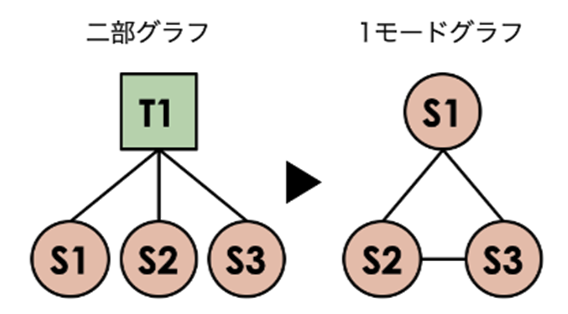
\includegraphics[width=0.9\linewidth]{graphs.png}
  \caption{2部グラフから1モードグラフへの変換}
  \label{fig:graphs}
 \end{center}
\end{figure}

また,2段の幅に跨る図は \verb|figure| 環境の替わりに \verb|figure*| 環境を利用すれば良い.

\subsection{表}

表は \verb|table| 環境を利用する\footnote{図と同様,2段の幅を使いたいときは \verb|table*| 環境を用いる.}.
表の例を表\ref{tab:competency} に示す.
表の直上に見出しを \verb|\caption| で指定し,\verb|\label| で付けたラベルを \verb|\ref| コマンドで参照する.

表の罫線はなるべく少なくすると見やすくなる.
罫線はもっとも上のものを二重線とし,左右の端には縦の罫線を描かないようにするとすっきりする.

\begin{table}[tb]
 \begin{center}
  \caption{コンピテンシーディクショナリの項目数}
  \label{tab:competency}
  \begin{tabular}{c|ccc}
   \hline\hline
   名称 & タスク & スキル & 関連知識\\
   \hline
   項目数 & 639 & 491 & 8843\\
   分類 & 203 & 150 & 3308\\
   \hline
  \end{tabular}
 \end{center}
\end{table}

\subsection{謝辞}

研究を進めたり卒業論文を作成したりしたときにお世話になった人(友人,知人,家族等)がいれば,謝辞を具体的に記して謝意を述べる.
また,指導教員には必ず謝辞を述べるものである.
謝辞は参考文献リストの直前に置き,\verb|acknowledgment| 環境を用いる.

この節の文章は敬体で良い.
例えば「○○教授には卒業論文作成全般にわたりご指導いただきました.深く感謝します.」
「○○氏には○○に関する重要な示唆をいただきましたので感謝します.」
「○○についての有用なデータをご提供いただいた○○氏に感謝します.」など\footnote{ここには具体的なことのみを記し,家族からの精神的なサポートなど抽象的なことについては書かない.}.

\subsection{参考文献}

卒業論文の最後には参考文献のリストを配置する.
ここは,卒業論文を執筆するにあたり著者が如何にたくさんの文献を読んだか,如何に深く調査をしたかをアピールする場所である.

\subsubsection{参考文献リスト}

参考文献リストには本文中で参照した文献のみを参照順(本文での出現順)に列挙する\footnote{BibTeXを利用すれば自動的に参照順のリストを生成してくれるので,執筆時に順序は気にしなくて良い.}.
その際,誌に掲載された記事や論文の場合\cite{newsweek2021,uetsugu2023},論文誌や国際会議の予稿集(Proceedings)に掲載された論文の場合\cite{miyashita2016},書籍の場合\cite{okumura2020,fukuchi2019}などについて \verb|references.bib| の通りに記述する.
これは BibTeX というシステムで処理されるファイルなので,他の場合の書式については``BibTeX''や``参考文献''などのキーワードで検索すると良いだろう.

なお \verb|main.tex| 中にある以下の2行によって参考文献リストが生成されるので,これらの行は削除しないこと.

\noindent
\verb|\bibliography{references}|
\verb|\bibliographystyle{junsrt}|

\ref{footnote}節で言及した通り,WWWサイトのURLは原則として参考文献ではなく脚注に記す.
これは,出版されている書籍や論文の「出版された」という事実やその内容が不変であるのに対して,WWW上の情報は内容が変更されたり削除されることがあるため参考文献に相応しくないと宮下が考えているからである.

\subsubsection{参考文献の参照}

本文中で参考文献を参照するときは \verb|\cite| コマンドを用いる.
巻末の参考文献リストにある番号が本文に挿入される.


\section{論文内容についての指針}

卒業論文とは,大学で学修した内容の集大成として取り組んだ卒業研究についてまとめ,報告するものである.
論文の内容について以下のような指針を示すので,提出前はもちろん執筆中にも適宜チェックリストとして活用してほしい\footnote{このリストは教員による卒業論文の評価尺度としても利用される.}.

また,執筆中の論文を他人(AIも含む)に読んでもらい助言をもらうことは非常に有効である.
その際にはこの指針も示し,このような視点でチェックしてもらうと良いだろう.

\subsection{基本的な書き方}

卒業論文の基本的な書き方について,以下のようなことに留意してほしい.
\begin{itemize}
 \item[□] 解決すべき課題を十分に具体化し明確にする
 \item[□] 研究の新規性や有用性,信頼性が読者に伝わるように記述する
 \item[□] 結論は明確に記す.その範囲や限界,問題点などを具体的に述べる
 \item[□] 一人称は「著者」を用いる(「私」とはしない)
 \item[□] 読みやすく理解しやすい文章を書く
 \item[□] 文脈から推測しないと理解できない文章を書かない
 \item[□] 飛躍のある文章や,逆に回りくどい文章を書かない
 \item[□] 極端な口語体など論文として不適当な表現は用いない
 \item[□] 一般的でない用語を未定義のまま使用しない
 \item[□] 内容を端的に表現する表題を付ける
 \item[□] 論文内容を適切に要約した概要を記す
 \item[□] 図表の説明はその内容を適切に表現するよう端的に記す
 \item[□] 図表の大きさや解像度などを適切にする
 \item[□] 他の論文や書籍等の引用や参照は参考文献リストに出典を明記する
 \item[□] WWWページへの参照はURLを脚注に記す
\end{itemize}

\subsection{新規性や有用性を明確にするために}

本ゼミの卒業論文では新規性はそれほど重要ではないが,いわゆる「車輪の再発明\footnote{広く知られている物事をもう一度最初からやり直すことをいう.すなわち,他の研究で既に明らかになっていることを再確認しただけの内容では卒業論文にならない.}」はできるだけ避けたい.
そのため,関連研究との相違を明確にすることが求められる.
また,有用性は重要であり,この研究の結果がどんな人をハッピーにするのか,ぜひアピールしてほしい.
その際,以下のようなことに注意すると良いだろう.
\begin{itemize}
 \item[□] 研究の中心となる問いを端的に説明する
 \item[□] 研究の背景や動機を述べ,問いの重要性を説明する
 \item[□] 従来の研究との関連(および相違)を充分に説明する
 \item[□] 既知の技術やアイデアと自分の考えを明確に分ける
 \item[□] 自分の考えの新規性や有用性を客観的に説明する
 \item[□] 新規性や有用性を主張するために必要十分な量の文献を参照する
 \item[□] 参考文献の数は10〜20件にする(数件では話にならないが,あまりに多いのも考えものである)
\end{itemize}



\section{おわりに}

この原稿では京都女子大学現代社会学部宮下ゼミの学生向けに,卒業論文のテンプレートを示した.
このテンプレートに足りないところや誤りがあればいつでも指摘してほしい.

すばらしい卒業論文が作成されることを期待しているし,あなたがそれを作成するための手助けは惜しまない.

\bibliography{references}
\bibliographystyle{ipsjunsrt}

\end{document}
